\documentclass[10pt,journal,compsoc]{IEEEtran}
\usepackage[T1]{fontenc}
\usepackage{graphicx}
\usepackage{amsmath,amssymb}
\usepackage{booktabs,array,tabularx,multirow}
\usepackage{microtype}
\usepackage[nocompress]{cite}
\usepackage{url}
\usepackage{xcolor}
\definecolor{ASVblue}{HTML}{3F6C9B}
\definecolor{ASVochre}{HTML}{B8753B}
\definecolor{ASVochreText}{HTML}{8C552A}
\definecolor{ASVgreen}{HTML}{4F7F5F}
\definecolor{ASVgray}{HTML}{6F6F6F}
\definecolor{ASVrule}{HTML}{D4D7D9}
\usepackage[hidelinks,hypertexnames=false]{hyperref}
\usepackage{tikz}
\usetikzlibrary{arrows.meta,positioning,fit,calc}
\usepackage{enumitem}
\usepackage{needspace}
\usepackage{algorithm}
\usepackage{algpseudocode}
\newcolumntype{Y}{>{\raggedright\arraybackslash}X}
\newcolumntype{L}[1]{>{\raggedright\arraybackslash}p{#1}}
\newcommand{\bit}{\mathrel{\equiv_{\mathrm{bits}}}}
\newcommand{\Simple}{\textsc{Simple}}
\newcommand{\Local}{\textsc{Local}}
\newcommand{\tighttable}{\renewcommand{\arraystretch}{1.10}\setlength{\tabcolsep}{4pt}}
\newcommand{\evidence}[1]{\textsf{#1}}
\setlist[enumerate]{leftmargin=*,itemsep=2pt,topsep=3pt}
\setlist[itemize]{leftmargin=*,itemsep=1pt,topsep=3pt}
\interdisplaylinepenalty=2500
\hyphenation{CUDA Vulkan pre-fill kernel back-end back-ends micro-batch}
\hypersetup{pdftitle={Reference-Compatible Parallel Execution for Quantized LLM Inference},pdfauthor={Chengzhan Li},pdfsubject={Reference-derived phase plans for quantized language-model execution}}
% Use the class's body size, leading, margins and column width.
\setlength{\textfloatsep}{11pt plus 2pt minus 2pt}
\setlength{\dbltextfloatsep}{11pt plus 2pt minus 2pt}
\setlength{\floatsep}{9pt plus 2pt minus 2pt}
\setlength{\dblfloatsep}{9pt plus 2pt minus 2pt}
\setcounter{topnumber}{3}
\setcounter{dbltopnumber}{2}
\renewcommand{\topfraction}{.90}
\renewcommand{\dbltopfraction}{.90}
\renewcommand{\textfraction}{.08}
\renewcommand{\floatpagefraction}{.80}
\renewcommand{\dblfloatpagefraction}{.80}
\raggedbottom

\newcommand{\StrongSTwoRows}{%
Q4\_K & q4 & 0.7370 & 0.9693 & [0.9576, 0.9885] \\
Q4\_K & q32 & 0.4731 & 0.6929 & [0.6803, 0.7029] \\
Q6\_K & q4 & 0.8205 & 0.9903 & [0.9624, 1.0102] \\
Q6\_K & q32 & 0.5829 & 0.7954 & [0.7473, 0.8708] \\
}


\newcommand{\ApplicationRows}{%
Qwen3-8B & 2.7274 & 2.6898 & 2.7287 & 2.6913 & 2.2726 & 2.2269 \\
Qwen3-14B & 4.6298 & 4.6022 & 4.6291 & 4.6028 & 3.4643 & 3.4268 \\
Llama-8B & 2.8879 & 2.8516 & 2.8874 & 2.8515 & 2.5631 & 2.5230 \\
}
\newcommand{\FactorRows}{%
8B & L/W; loop4 fixed & 0.997913 & [0.995370, 0.999576] \\
8B & L/W; packed fixed & 0.998717 & [0.995953, 1.000570] \\
8B & P/L4; W fixed & 0.983648 & [0.980236, 0.988654] \\
8B & P/L4; L fixed & 0.984440 & [0.981228, 0.989391] \\
14B & L/W; loop4 fixed & 0.996957 & [0.994726, 0.999092] \\
14B & L/W; packed fixed & 0.998881 & [0.997093, 1.000227] \\
14B & P/L4; W fixed & 0.990130 & [0.988351, 0.992804] \\
14B & P/L4; L fixed & 0.992041 & [0.990754, 0.993985] \\
}
\newcommand{\QThreeTwoRows}{%
\texttt{W\_REF1L\_M} & 124.182883 & 7.7614 & 343.310 & 425.997 \\
\texttt{W\_REF1G\_M} & 117.208239 & 7.3255 & 329.630 & 409.576 \\
\texttt{L\_REF1L\_M} & 124.100017 & 7.7563 & 344.139 & 428.399 \\
\texttt{L\_REF1G\_M} & 117.143582 & 7.3215 & 328.455 & 412.088 \\
\texttt{W\_REF1L\_D4} & 147.748374 & 9.2343 & 396.385 & 478.532 \\
\texttt{L\_REF1G\_D4} & 133.543739 & 8.3465 & 365.014 & 455.562 \\
}
\newcommand{\QEightRows}{%
W-L4-k3 & 185.311926 & 1.447749 \\
W-L4-k7 & 210.950040 & 1.648047 \\
W-P-k3 & 183.631913 & 1.434624 \\
W-P-k7 & 209.005981 & 1.632859 \\
L-L4-k3 & 183.035577 & 1.429965 \\
L-L4-k7 & 209.736406 & 1.638566 \\
L-P-k3 & 183.366590 & 1.432551 \\
L-P-k7 & 208.263503 & 1.627059 \\
}
\newcommand{\QEightSecondaryRows}{%
W-P-k7 / W-L4-k7 & 0.990784 & [0.981234, 1.000085] \\
L-P-k7 / L-L4-k7 & 0.992977 & [0.981103, 1.007912] \\
L-L4-k7 / W-L4-k7 & 0.994247 & [0.983947, 1.004513] \\
L-P-k7 / W-P-k7 & 0.996448 & [0.985822, 1.009280] \\
}

\newcommand{\AmperePilotRows}{%
Whole / loop4 & 12.039 & 13.824 \\
Whole / packed & 11.897 & 13.598 \\
Local / loop4 & 11.997 & 13.800 \\
Local / packed & 11.879 & 13.549 \\
}

\ifdefined\arxivReadable% Author-preprint typography for reference-compatible parallel execution, 2026-11-10.
% NOT an official IEEE/TPDS stylesheet. main.tex without arxivReadable
% retains the Computer Society journal typography and affiliation footnote.
% No change to IEEEtran.cls, page dimensions, column widths or body leading.
\usepackage{mathpazo}
\renewcommand{\sfdefault}{ppl}
\urlstyle{same}
\makeatletter
% Match abstract and headings to the body family. Keep the label bold,
% the abstract itself regular; increase the front-matter text modestly.
\renewcommand{\@IEEEabskeysecsize}{\fontsize{9}{11}\selectfont}
% Reader-preprint title-to-body separation; keep body leading untouched.
\def\@IEEENORMtitlevspace{1.5\baselineskip}
\def\@IEEEMINtitlevspace{1\baselineskip}
\makeatother
% A quiet separator replaces the Computer Society ornamental diamond only
% in this reader-oriented preprint. The strict journal build is unchanged.
\renewcommand{\IEEEcompsocdiamondline}{\rule{0.45\textwidth}{0.35pt}}

% The reading edition uses a plain initial; the journal edition keeps the class drop cap.
\renewcommand{\IEEEPARstart}[2]{#1#2}
\fi
\begin{document}
\ifdefined\arxivReadable
\title{Reference-Compatible Parallel Execution\\for Quantized LLM Inference}
\author{Chengzhan Li\\[3pt]\small University of Electronic Science and Technology of China\\Chengdu, China\\\href{mailto:chengzhan.li@std.uestc.edu.cn}{chengzhan.li@std.uestc.edu.cn}}
\else
\title{Reference-Compatible Parallel Execution for Quantized LLM Inference}
\author{Chengzhan Li\IEEEcompsocitemizethanks{\IEEEcompsocthanksitem C. Li is with the University of Electronic Science and Technology of China, Chengdu, China. E-mail: chengzhan.li@std.uestc.edu.cn.}}
\fi
\markboth{REFERENCE-COMPATIBLE PARALLEL EXECUTION}{}
\IEEEtitleabstractindextext{\begin{abstract}Batching a quantized language model can change its numerical output even when token positions and causal masks stay the same. We introduce reference-derived phase plans for parallel inference that retains an established deployment's numerical behavior. A plan binds the prompt producer, physical KV range, arithmetic recipe and ownership of outputs and state. It places cuts around whole graphs or within attention, while packing independent arithmetic groups into wider operations. Implementations on CUDA and Vulkan cover Qwen, Llama and SmolLM2, including a mixed-Q4 32B model. On Linux/A5000, compatible speculative applications reduce resident-service time by 17.21\%, 25.54\% and 11.52\% against the fastest measured fixed target-only control for Qwen3-8B, Qwen3-14B and Llama-8B. Separate balanced experiments attribute 0.80\%--1.64\% to Q8 projection packing; local cuts contribute smaller, geometry-dependent gains. For 32B mixed quantization, independent-channel grouping reduces ordinary service time by 5.61\% relative to a graph-level scalar-column loop. Eight-query execution also lowers aggregate cost at equal work, while longer live proposals add enough work to favor the shorter configuration. Phase plans thus preserve reference-sensitive computation while exposing parallel work, with complete-request costs guiding the choice of execution strategy.
\end{abstract}
\begin{IEEEkeywords}Parallel inference, quantized language models, numerical compatibility, execution planning, speculative decoding.\end{IEEEkeywords}}
\maketitle
\IEEEdisplaynontitleabstractindextext
\section{Introduction}
\label{sec:intro}
Quantized language-model runtimes expose parallel work whenever the next inputs are already known. Prompt processing supplies a sequence of queries; speculative decoding supplies proposed continuations for batched target verification~\cite{leviathan2023,chen2023}. The execution can use this parallelism without changing the mathematical model, yet produce different floating-point outputs. Batch width can change activation quantization, reduction organization or the physical range consumed by attention. A causal mask fixes which keys are logically visible, but does not fix those numerical operations.

An established deployment needs more than repeatable output: it needs compatibility with the execution already used by regression tests and stateful continuations. That execution includes the prompt producer, incoming KV state and requested output rows, as well as weights and numerical libraries. The optimization problem is to retain their numerical behavior across prefill, continuation, verification and commit while reorganizing known-query work.

There are several ways to control numerical execution. Batch-invariant operators fix reduction choices~\cite{thinkingmachines}; arithmetic reconstruction and compiler enforcement can preserve existing library behavior~\cite{taming}; deterministic engines can relate state invariants to kernel contracts~\cite{vosti}. Fixed-shape schedules and verified speculation provide other system designs~\cite{corun,llm42}. We study compatibility with a quantized deployment fixed before optimization. Parallelism comes from reorganizing independent work around its reference arithmetic.

\begin{figure*}[t]
\centering
% One measured example throughout. Widths encode query grouping, never time.
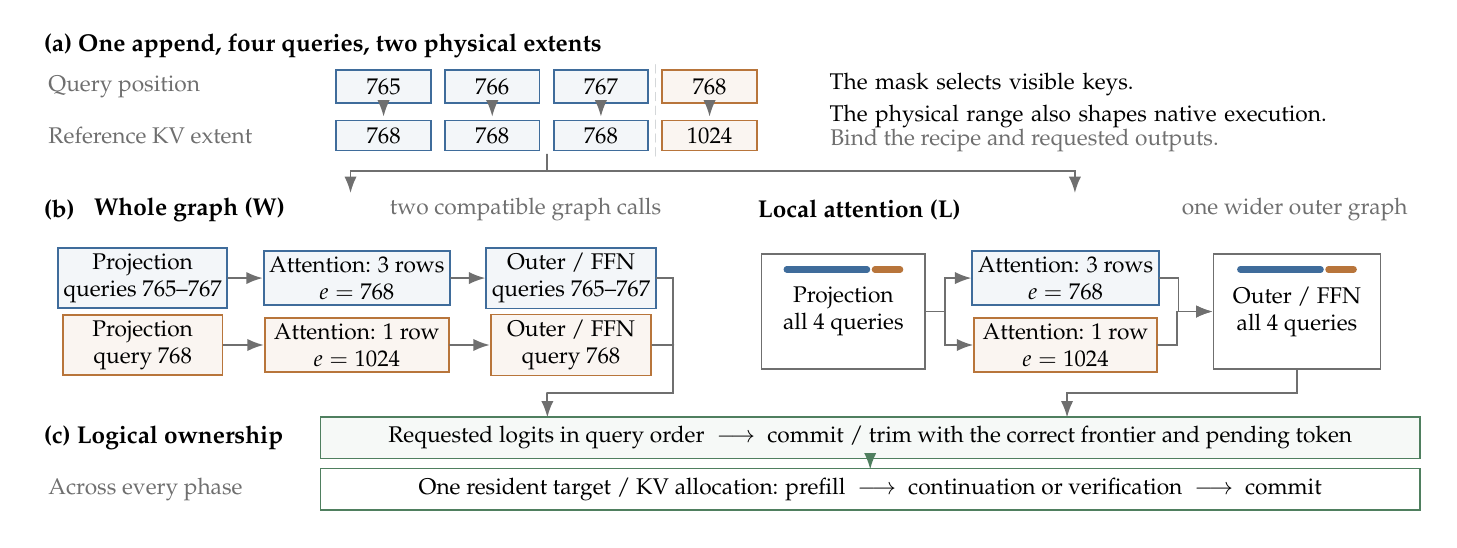
\begin{tikzpicture}[x=1cm,y=1cm,font=\fontsize{8.2}{9.7}\selectfont,
  >=Latex,line cap=round,
  flow/.style={->,draw=ASVgray,line width=.65pt},
  stateflow/.style={->,draw=ASVgreen,line width=.65pt},
  head/.style={font=\fontsize{8.8}{10.2}\selectfont\bfseries,anchor=west},
  three/.style={draw=ASVblue,fill=ASVblue!6,line width=.65pt,align=center,inner sep=2pt},
  one/.style={draw=ASVochre,fill=ASVochre!7,line width=.65pt,align=center,inner sep=2pt},
  wide/.style={draw=ASVgray,fill=white,line width=.65pt,align=center,inner sep=3pt}]
\path[use as bounding box] (0,0) rectangle (17.8,6.25);
\node[head] at (.08,6.02) {(a) One append, four queries, two physical extents};
\node[anchor=west,text=ASVgray] at (.14,5.50) {Query position};
\node[anchor=west,text=ASVgray] at (.14,4.88) {Reference KV extent};
\foreach \i/\pos/\ext in {0/765/768,1/766/768,2/767/768}{
  \node[three,minimum width=1.20cm,minimum height=.42cm] at (4.52+1.38*\i,5.50) {\pos};
  \draw[flow] (4.52+1.38*\i,5.26)--(4.52+1.38*\i,5.12);
  \node[three,minimum width=1.20cm,minimum height=.38cm] at (4.52+1.38*\i,4.88) {$\ext$};
}
\node[one,minimum width=1.20cm,minimum height=.42cm] at (8.66,5.50) {768};
\draw[flow] (8.66,5.26)--(8.66,5.12);
\node[one,minimum width=1.20cm,minimum height=.38cm] at (8.66,4.88) {$1024$};
\draw[ASVrule,densely dashed] (7.97,4.62)--(7.97,5.80);
\node[anchor=north west,align=left,text width=7.35cm] at (10.07,5.80) {The mask selects visible keys.\\[2pt]The physical range also shapes native execution.};
\node[anchor=west,text=ASVgray] at (10.07,4.82) {Bind the recipe and requested outputs.};
% Branch to two alternative lowerings of exactly the same four rows.
\draw[ASVgray,line width=.65pt] (6.60,4.64)--(6.60,4.43);
\draw[flow] (6.60,4.43)--(4.10,4.43)--(4.10,4.15);
\draw[flow] (6.60,4.43)--(13.30,4.43)--(13.30,4.15);
\node[head] at (.08,3.94) {(b)};
\node[head] at (.72,3.94) {Whole graph (W)};
\node[anchor=east,text=ASVgray] at (8.17,3.94) {two compatible graph calls};
\node[head] at (9.15,3.94) {Local attention (L)};
\node[anchor=east,text=ASVgray] at (17.65,3.94) {one wider outer graph};
% Whole graph: both projection and outer work are split along with attention.
\node[three,minimum width=2.03cm,minimum height=.61cm] (wp3) at (1.46,3.07) {Projection\\queries 765--767};
\node[three,minimum width=2.34cm,minimum height=.61cm] (wa3) at (4.18,3.07) {Attention: 3 rows\\$e=768$};
\node[three,minimum width=2.04cm,minimum height=.61cm] (wf3) at (6.90,3.07) {Outer / FFN\\queries 765--767};
\node[one,minimum width=2.03cm,minimum height=.61cm] (wp1) at (1.46,2.22) {Projection\\query 768};
\node[one,minimum width=2.34cm,minimum height=.61cm] (wa1) at (4.18,2.22) {Attention: 1 row\\$e=1024$};
\node[one,minimum width=2.04cm,minimum height=.61cm] (wf1) at (6.90,2.22) {Outer / FFN\\query 768};
\draw[flow] (wp3)--(wa3);\draw[flow] (wa3)--(wf3);
\draw[flow] (wp1)--(wa1);\draw[flow] (wa1)--(wf1);
% Local attention: the same blue/ochre partition is confined to attention.
\node[wide,minimum width=2.08cm,minimum height=1.46cm] (lp) at (10.36,2.645) {Projection\\all 4 queries};
\node[three,minimum width=2.32cm,minimum height=.61cm] (la3) at (13.18,3.07) {Attention: 3 rows\\$e=768$};
\node[one,minimum width=2.32cm,minimum height=.61cm] (la1) at (13.18,2.22) {Attention: 1 row\\$e=1024$};
\node[wide,minimum width=2.12cm,minimum height=1.46cm] (lf) at (16.12,2.645) {Outer / FFN\\all 4 queries};
\foreach \x in {10.36,16.12}{
 \draw[ASVblue,line width=2.3pt] (\x-.72,3.18)--(\x+.30,3.18);
 \draw[ASVochre,line width=2.3pt] (\x+.40,3.18)--(\x+.72,3.18);
}
\draw[flow] (lp.east)--++(.24,0)|-(la3.west);
\draw[flow] (lp.east)--++(.24,0)|-(la1.west);
\draw[flow] (la3.east)--++(.24,0)|-(lf.west);
\draw[flow] (la1.east)--++(.24,0)|-(lf.west);
% Either lowering returns the same logical outputs into one owned state.
\draw[ASVgray,line width=.65pt] (wf3.east)--(8.20,3.07)--(8.20,1.61)--(6.60,1.61);
\draw[ASVgray,line width=.65pt] (wf1.east)--(8.20,2.22);
\draw[flow] (6.60,1.61)--(6.60,1.30);
\draw[flow] (lf.south)--(16.12,1.61)--(13.20,1.61)--(13.20,1.30);
\node[head] at (.08,1.04) {(c) Logical ownership};
\node[draw=ASVgreen,fill=ASVgreen!5,line width=.65pt,minimum width=13.96cm,minimum height=.49cm,align=center] at (10.70,1.04)
 {Requested logits in query order $\;\longrightarrow\;$ commit / trim with the correct frontier and pending token};
\node[anchor=west,text=ASVgray] at (.14,.39) {Across every phase};
\node[draw=ASVgreen,line width=.65pt,minimum width=13.96cm,minimum height=.45cm,align=center] at (10.70,.39)
 {One resident target / KV allocation: prefill $\;\longrightarrow\;$ continuation or verification $\;\longrightarrow\;$ commit};
\draw[stateflow] (10.70,.79)--(10.70,.64);
\end{tikzpicture}

\caption{Reference-derived phase execution for one measured append. (a) Positions 765--768 require extents 768, 768, 768 and 1024. Blue and ochre track the two groups. (b) Whole lowering splits the graph; local lowering confines the split to attention and retains wider outer work. (c) Both preserve logical outputs and the frontier on one resident state. Arrows denote dependencies, not measured durations.}
\label{fig:overview}
\end{figure*}

A \emph{reference-derived phase plan} connects these requirements (Fig.~\ref{fig:overview}). Source analysis and native tests establish an arithmetic recipe; the runtime reads cache occupancy, head and padding to assign each query its physical range. In the illustrated append, the first three queries require extent 768 and the fourth requires 1024. The plan executes these compatible groups while keeping the target and KV resident. Requested vectors remain associated with their logical rows, preserving the frontier needed after a commit or trim.

Two lowerings implement these requirements. Whole-graph lowering places cuts around an entire graph and can realign subsequent groups after a physical boundary. Local-attention lowering applies the cuts within attention, retaining broader projection and feed-forward work. Projection organization is a separate choice. A backend loop reuses a reference-compatible small-column arithmetic path; independent-channel packing executes several such groups together. For the affected CUDA Q8 path, the preserved group has four columns. The mixed Q4\_K/Q6\_K extension retains scalar-column arithmetic and parallelizes the independent columns. The arithmetic group is type- and backend-specific; the physical-prefix and state interface is shared.

The evaluation covers three model families and both backends. A Linux/Ampere deployment rebuilds the numerical modules and establishes its own reference. Frozen CUDA rules transfer between grouped-query and multi-head attention structures; a typed recipe extension supports a 32B mixed-quantization model. Comparisons stay within each deployment's numerical contract.

On Linux/A5000, compatible speculative applications reduce resident service by 17.21\%, 25.54\% and 11.52\% relative to the fastest measured fixed target-only control for Qwen3-8B, Qwen3-14B and Llama-8B. These are application gains. Balanced factorial experiments isolate packing's 0.80\%--1.64\% increment and the smaller, geometry-dependent contribution of local cuts. In a 32B target-only deployment, channel grouping saves 5.61\% relative to graph-level scalar-column execution.

The contributions are a phase-plan interface that composes producer, physical-prefix, arithmetic and state requirements; whole and local implementations with reference-compatible Q8 and mixed-Q4 groups; and an evaluation that separates structural transfer, implementation increments and complete-service value. Ordinary generation and speculative verification use the same interface, with strong simple controls and full request costs determining the useful configuration.

\section{Reference Semantics and Physical Execution}
\label{sec:reference}
\subsection{The fixed reference is a deployment execution}
Let $R_d$ denote the execution fixed for deployment $d$ before candidate optimization. Its identity includes model and tokenizer bytes, prompt formatting, numerical modules, device placement, KV type and capacity, producer calls, requested outputs, sampling and stopping semantics. A candidate $F_d$ may change how known queries are scheduled while preserving the observations required by $R_d$.

For a materialized token prefix $x$, write $\ell^R(x)$ for its full binary32 target vocabulary vector and $K^R(x)$ for its active KV state in canonical logical order. The numerical target at a declared observation boundary is
\begin{equation}
 \ell^F(x)\bit\ell^R(x),\qquad K^F(x)\bit K^R(x),
 \label{eq:contract}
\end{equation}
with matching logical positions, frontier and termination behavior. Equality is checked on complete values, without a tolerance. Active state excludes unused storage, whose bytes need not describe a logical token. 

The producer is phase-specific. The CUDA references use a whole-prompt caller with physical microbatch one and last-only prompt output. The Vulkan reference retains its original physical microbatch 128 producer, with the declared outer prompt chunks, then scalar continuation. Replacing that producer with scalar prefill would change the numerical reference. Likewise, a context's output reservation is a capacity declaration, not the number of occupied query rows in a call.

Speculative execution evaluates prefixes that may later be rejected. Each requested target vector is compared with an independent reference forced through the same prefix after the original producer. An autonomous reference, receiving only the original prompt, supplies the emitted-token and stopping oracle. This separates numerical correspondence on a candidate branch from the free-generation endpoint. Draft logits and proposals can change; the target must satisfy the reference contract on the prefixes it actually evaluates.

\subsection{The physical range participates in numerical execution}
A measured Llama example illustrates why logical equivalence alone is insufficient. Four queries at positions 765--768 required extents $[768,768,768,1024]$ under the single-query reference. An unsplit batch used 1024 for every row. Captured visible Q, K, V, QK and effective probability prefixes were identical, but the AV outputs differed. Cropped-range and padded-range replays reproduced the respective reference and batched results~\cite{records}. The earliest saved full-vector difference preceded the first emitted-token difference, at positions 29 and 81 respectively.

The intervention identifies a physical execution requirement. On Vulkan, extent changes continuity and dispatch as well, so the intervention identifies their combined physical effect. A second mechanism concerns activation arithmetic: affected Q8-weight projections use F32 activations on the scalar path, but a wider path can introduce Q8\_1 activation quantization. Retaining the F32 path restores the corresponding arithmetic condition. In a Llama control, that repair alone matched emitted tokens while 99 committed full vectors still differed; the physical-prefix repair removed the remaining discrepancies. The mechanisms are separable and have different backend implementations.

The planner derives cuts from live state. At physical head 767, a Qwen witness requires extents $[768,1024,1024,1024]$; the resulting whole-graph $1+3$ plan and local-attention counterpart both preserve the independent reference. The same extent rule handles this witness and the $3+1$ example in Fig.~\ref{fig:overview}.

\subsection{State and requested outputs connect the phases}
The state at a commit contains more than a token list. It includes the materialized prefix, its active KV, the logical frontier vector and any emitted token that has not yet been materialized. A cap or end-of-generation stop can leave the last emitted token pending. Verification can instead append several proposals and then trim rejected state.

Consequently, the last physical output buffer is not always the frontier of the retained logical prefix. The executor must associate requested vectors with their logical rows and preserve the required one before another native call overwrites scratch storage. It must also materialize a pending correction or bonus token exactly when the next phase requires it. These ownership rules make a compatible operator usable in a complete inference transaction.

\begin{table}[t]
\centering\footnotesize\tighttable
\caption{Information bound by a phase plan. Source qualification establishes the arithmetic recipe; live extraction supplies the current geometry and ownership.}
\label{tab:requirements}
\begin{tabularx}{\columnwidth}{@{}L{1.70cm}Y@{}}\toprule
Requirement & Effect on execution\\\midrule
Producer and phase & Retain the original incoming state and phase-specific numerical behavior.\\
Physical prefix & Read occupied slots, head and padding; bind each row's reference extent.\\
Typed arithmetic & Match activation, dot/reduction, stride, placement and dispatch requirements.\\
Requested rows & Preserve the original mask and own outputs by logical position.\\
Commit state & Maintain active KV, trim frontier, pending token and native stopping.\\
Reuse identity & Include effective geometry and phase policy in graph-reuse checks.\\\bottomrule
\end{tabularx}
\end{table}

\section{Reference-Derived Phase Plans}
\label{sec:method}
\subsection{Separate arithmetic qualification from per-call planning}
A backend recipe describes the operator conditions that preserve the deployment reference: weight and activation types, reduction organization, supported shapes and strides, placement and output layout. We establish these conditions through source analysis, own-path replay and controlled comparisons with independent reference operands. Descriptor guards select recipes whose numerical correspondence is established separately through native tests.

The planner combines the recipe with sequence ownership, occupied slots, physical head, capacity and padding. In the supported dense, nonwrapping append profile, occupied cells form the logical prefix and the physical head agrees with its end. The extractor checks this correspondence and rejects shifted, wrapped or holey states.

For first physical slot $H$, query row $i$, cache capacity $N$ and padding $P$, this profile gives
\begin{equation}
 e_i=\min\!\left(N,\max\!\left(P,P\left\lceil\frac{H+i+1}{P}\right\rceil\right)\right).
 \label{eq:extent}
\end{equation}
Each row carries its position, $e_i$, admitted arithmetic class and requested-output flag. The class is normally constant within one attention graph, while the extent changes at a physical boundary. Graph-reuse identity includes the recipe, per-row geometry and phase policy as well as the outer shape.

\subsection{Group compatible queries and place the cuts}
Let $\kappa_i$ contain a row's physical extent and recipe class. Whole-graph lowering (W) takes maximal adjacent runs of equal $\kappa_i$, subject to the native width bound $W_{\max}$. For constant-key run lengths $r_1,\ldots,r_m$, its minimum number of contiguous calls is
\begin{equation}
 G_{\min}=\sum_{j=1}^{m}\left\lceil r_j/W_{\max}\right\rceil.
 \label{eq:groups}
\end{equation}
Every key change forces a cut, and each run needs at least the stated number of bounded calls. Taking the longest allowed prefix of each run attains this grouping bound. Runtime also depends on cut placement and the backend implementation of each group.

Whole lowering executes projection, attention and feed-forward work for each compatible call. After a boundary, it can restart full-width calls rather than preserve the remainder of an arbitrary outer chunk. We retain this rechunking behavior as a strong simple implementation.

Local lowering (L) keeps the outer graph wider and forms compatible groups inside attention. Q, K, V and mask views use the appropriate reference extent. The adapter supplies the strides and, when required, contiguous mask materialization expected by the admitted backend. Attention outputs rejoin in query order, so projection and feed-forward operations outside the cut can use the wider query group. Native attention may further tile a compatible group according to its qualified recipe. Local cuts preserve parallel work around attention; they do not remove dependencies between autoregressively generated tokens.

The grouping pass is linear in the number of query rows. The current dense-cache validator also inspects the occupied prefix. Both extraction and grouping remain in the measured service, together with native dispatch and required synchronization.

\begin{algorithm}[t]
\caption{Execute a reference-derived phase}
\label{alg:plan}
\begin{algorithmic}[1]
\Require Live target/KV owner $S$, phase $p$, known rows $Q$, original requested-row mask $O$, admitted recipe $a$
\State Check phase, capacity, cache ownership and support of $a$
\State Extract physical-prefix requirements $\{e_i\}$ from $S$
\State Form compatible runs under $(e_i,a)$
\State Lower runs to whole-graph calls or local attention views
\For{each native call in logical order}
 \State Execute the selected arithmetic and original output requests
 \State Synchronize; store requested vectors by logical row
 \State Check successful append and expected physical execution
\EndFor
\State Commit or trim with the owned logical frontier and pending token
\State On native failure, invalidate the owner for further execution
\end{algorithmic}
\end{algorithm}

\subsection{Preserve arithmetic within groups, parallelize between groups}
\label{sec:recipes}
Projection organization is independent of cut scope. Consider $X\in\mathbb{R}^{K\times q}$, containing $q$ query columns, and a shared weight matrix. A recipe specifies an arithmetic group width $a$ whose native computation matches the reference. When $q=ag$, packing exposes the group index as an independent dimension:
\begin{equation}
 \widetilde X_{k,c,j}=X_{k,aj+c},\quad
 \widetilde X\in\mathbb{R}^{K\times a\times g}.
 \label{eq:packing}
\end{equation}
The backend computes each group with the admitted inner organization; the result is restored to logical column order. Each supported reshape is bound to the tensor layout and backend dispatch validated for that recipe.

\begin{figure*}[t]
\centering% Dependency/operation organization only: vertical spacing is not elapsed time.
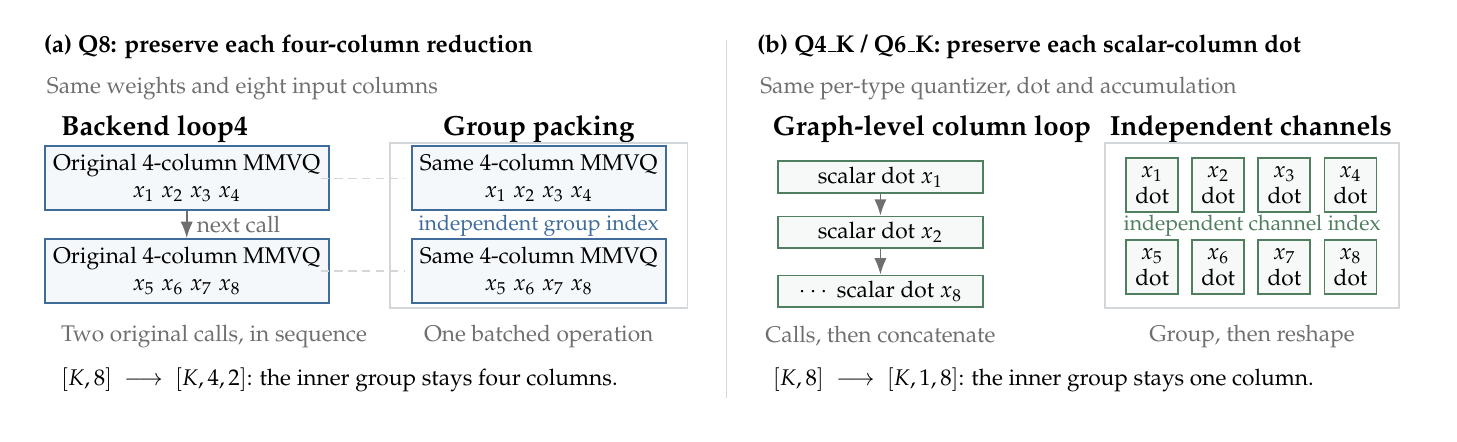
\begin{tikzpicture}[x=1cm,y=1cm,font=\fontsize{8.2}{9.6}\selectfont,>=Latex,
 flow/.style={->,draw=ASVgray,line width=.65pt},
 inner/.style={draw=ASVblue,fill=ASVblue!5,line width=.65pt,align=center,inner sep=3pt},
 scalar/.style={draw=ASVgreen,fill=ASVgreen!5,line width=.65pt,align=center,inner sep=2pt},
 head/.style={anchor=west,font=\fontsize{8.8}{10.2}\selectfont\bfseries}]
\path[use as bounding box] (0,0) rectangle (17.8,4.90);
\draw[ASVrule] (8.88,.20)--(8.88,4.74);
\node[head] at (.08,4.66) {(a) Q8: preserve each four-column reduction};
\node[head] at (9.14,4.66) {(b) Q4\_K / Q6\_K: preserve each scalar-column dot};
\node[anchor=west,text=ASVgray] at (.12,4.13) {Same weights and eight input columns};
\node[anchor=west,text=ASVgray] at (9.18,4.13) {Same per-type quantizer, dot and accumulation};
\node[anchor=west,font=\bfseries] at (.30,3.61) {Backend loop4};
\node[anchor=center,font=\bfseries] at (6.49,3.61) {Group packing};
\node[inner,minimum width=3.28cm,minimum height=.63cm] (g1) at (2.02,2.99) {Original 4-column MMVQ\\$x_1\;x_2\;x_3\;x_4$};
\node[inner,minimum width=3.28cm,minimum height=.63cm] (g2) at (2.02,1.81) {Original 4-column MMVQ\\$x_5\;x_6\;x_7\;x_8$};
\draw[flow] (g1.south)--(g2.north) node[midway,right,text=ASVgray] {next call};
\node[draw=ASVrule,line width=.65pt,minimum width=3.78cm,minimum height=2.10cm] (pack) at (6.49,2.39) {};
\node[inner,minimum width=3.18cm,minimum height=.63cm] (p1) at (6.49,2.99) {Same 4-column MMVQ\\$x_1\;x_2\;x_3\;x_4$};
\node[inner,minimum width=3.18cm,minimum height=.63cm] (p2) at (6.49,1.81) {Same 4-column MMVQ\\$x_5\;x_6\;x_7\;x_8$};
\node[text=ASVblue,font=\fontsize{7.7}{9}\selectfont] at (6.49,2.39) {independent group index};
\draw[ASVrule,densely dashed] (3.72,2.99)--(4.78,2.99);
\draw[ASVrule,densely dashed] (3.72,1.81)--(4.78,1.81);
\node[anchor=west,text=ASVgray] at (.30,.98) {Two original calls, in sequence};
\node[anchor=center,text=ASVgray] at (6.49,.98) {One batched operation};
\node[anchor=west] at (.30,.43) {$[K,8]\ \longrightarrow\ [K,4,2]$: the inner group stays four columns.};
% Mixed Q4: same visual distinction, but the indivisible recipe is scalar.
\node[anchor=west,font=\bfseries] at (9.34,3.61) {Graph-level column loop};
\node[anchor=west,font=\bfseries] at (13.62,3.61) {Independent channels};
\node[scalar,minimum width=2.60cm,minimum height=.40cm] (s1) at (10.83,3.00) {scalar dot $x_1$};
\node[scalar,minimum width=2.60cm,minimum height=.40cm] (s2) at (10.83,2.30) {scalar dot $x_2$};
\node[scalar,minimum width=2.60cm,minimum height=.40cm] (s8) at (10.83,1.55) {$\cdots$ scalar dot $x_8$};
\draw[flow] (s1.south)--(s2.north);\draw[flow] (s2.south)--(s8.north);
\node[draw=ASVrule,line width=.65pt,minimum width=3.74cm,minimum height=2.10cm] at (15.55,2.39) {};
\foreach \i/\x/\y in {1/14.28/2.90,2/15.12/2.90,3/15.96/2.90,4/16.80/2.90,5/14.28/1.86,6/15.12/1.86,7/15.96/1.86,8/16.80/1.86}{
 \node[scalar,minimum width=.66cm,minimum height=.68cm] at (\x,\y) {$x_{\i}$\\dot};
}
\node[text=ASVgreen,font=\fontsize{7.7}{9}\selectfont] at (15.55,2.38) {independent channel index};
\node[anchor=center,text=ASVgray] at (10.83,.98) {Calls, then concatenate};
\node[anchor=center,text=ASVgray] at (15.55,.98) {Group, then reshape};
\node[anchor=west] at (9.34,.43) {$[K,8]\ \longrightarrow\ [K,1,8]$: the inner group stays one column.};
\end{tikzpicture}

\caption{Arithmetic is preserved within each group. (a) Loop4 invokes four-column groups sequentially; packing exposes them to one batched operation. (b) The mixed-Q4 control uses scalar-column calls and concatenation; grouping exposes the columns as independent channels. Quantizer, stride and dispatch remain bound to the qualified recipe. Layout denotes operation organization, not timing.}
\label{fig:arithmetic}
\end{figure*}

\subsubsection{CUDA Q8 recipe}
For affected Q8\_0 projections with F32 input, the implementation preserves the existing small-column MMVQ path with $a=4$. The backend-loop4 control quantizes the input and invokes the original small-column specialization for successive groups and the supported tail. Packing uses $[K, 4,g]$ views for eligible multi-group work and shares the weight across groups. The four-column reduction within a group is retained. Tails retain the native path validated for their shape.

This distinction matters for verification. A $k=3$ transaction requests at most four target positions and does not enter the wider packing route. A $k=7$ transaction can request eight positions and two independent four-column groups. The draft's prefill microbatch, denoted D1 or D4 in the experiments, is a separate parameter.

\subsubsection{Mixed Q4\_K/Q6\_K recipe}
The 32B model contains Q4\_K, Q6\_K and F32 tensors. Its affected mixed-quantized projections retain the original scalar-column path, so $a=1$. One implementation creates a view, scalar matrix operation and output concatenation for each column. The grouped implementation maps the same columns to $[K, 1,q]$ and executes them as independent channels, then reshapes the output to the caller's layout. The original per-type dot functions, activation quantizer and accumulation organization are preserved. The Q8 four-column guard remains unchanged.

The mixed-Q4 service implementation changes graph lowering and compiled into a new core archive; the recorded CUDA numerical objects remain byte-identical. Qualification uses actual full-model operands and an independent scalar reference, followed by full-model state and output checks. The full-service control is graph-level scalar-column execution using the same per-type arithmetic.

\subsubsection{Vulkan mapping}
Affected Q8-weight projections retain F32 activation input rather than selecting the wider Q8\_1 path. Attention preserves the admitted scalar-equivalent AV reduction and its stride/dispatch requirements, including the p021 mapping used by the resident implementation. The physical-prefix grouping principle is shared with CUDA; its native arithmetic implementation is backend-specific. This supports two-query verification and wider known-query append with the original prompt producer.

\subsection{Keep one state owner across phases}
The phase interface binds each plan to the existing target context. Prefill, ordinary continuation and verification share one resident target/KV owner; a phase transition changes the execution policy while retaining that allocation.

The caller's requested-row mask is preserved through splitting. After a native call has made the requested vectors available, the executor copies them into logical output slots before subsequent calls can reuse scratch memory. The accepted prefix can then select its frontier even when a later physical row was rejected. A commit or trim updates active state and pending-token bookkeeping together. Reset returns the owner to its declared initial condition; an execution failure prevents further use of a partially updated owner.

Clean execution performs planning, synchronization, output copies and state operations. Independent-reference replay and heavy internal-state capture are confined to qualification runs using the same numerical build and transaction semantics.

\subsection{Why the requirements compose}
The compositional argument has three obligations. A phase begins from reference-compatible active state and producer history. Each native group uses a recipe that preserves the required outputs and state update for its supported descriptor. Finally, logical output ownership and the transaction rules retain the reference frontier and committed state at the next boundary. Under these obligations, an induction over groups and phase boundaries preserves the contract in Eq.~\eqref{eq:contract}.

This argument identifies what must be checked when a recipe or lowering changes. Source analysis, actual-operand comparisons and full-model tests evaluate these obligations in the listed deployments. Descriptor guards enforce the resulting supported domain.

\section{Implementation and Evaluation}
\label{sec:eval}
\subsection{Deployments and comparison structure}
The implementations extend a pinned llama.cpp/ggml runtime, with commit-bound numerical modules, model bytes, tokenizer and prompt templates~\cite{records}. CUDA studies use a Windows RTX 5070 Ti Laptop GPU and a Linux RTX A5000; Vulkan studies use an Intel Arc B570. Models cover Qwen3, Llama and SmolLM2~\cite{qwen3,llama3,smol}. Each deployment fixes its own reference before candidate comparisons. The Linux deployment rebuilds the reference and candidate numerical modules from source, including the CUDA, base and CPU backends.

The evaluated state profile is dense single-sequence inference, with F16 KV, greedy output and no FlashAttention. Outer known-query work reaches 32 positions; the later CUDA verification study supports eight occupied query rows. Natural service panels use C1024, and the final Vulkan append interface is also checked at C4096. Table~\ref{tab:panels} binds the measured profiles, producer semantics and cost windows.

W/L denotes whole/local cuts, and L4/P denotes backend-loop4/packed projections. Q8\_0 names weight quantization; $q$ is the number of query rows and $k$ the number of draft proposals. M denotes target-only generation. D4 sets draft prefill microbatch UB4; it does not set $k$. Unless stated otherwise, $k=3$. All applicable controls receive the same legal numerical, residency and graph-reuse improvements. Ordinary generation remains an application alternative and loads no idle draft in the latest Linux panels.

\begin{table*}[t]
\centering\footnotesize\tighttable
\caption{Main evidence panels. Counts exclude separate numerical qualification. A repeated timing is not an additional independent task. The 8B and 14B Linux transfer panels share the same sixteen task identities. Source and full control tables are in the supplement.}
\label{tab:panels}
\begin{tabularx}{\textwidth}{@{}L{2.00cm}L{2.22cm}L{2.40cm}L{1.64cm}L{1.40cm}Y@{}}\toprule
Panel & Platform / model & Compared paths & Root / repetition unit & Measured + warm & Observation and cost window\\\midrule
Linux service & A5000; Qwen3-8B, 14B & Four target-only M; W-L4-D4, L-P-D4 & 16 exposed roots; 4 sessions & $384+48$ each & Resident service plus actual startup, request burst and worker clocks.\\
Llama service & A5000; Llama-8B/1B & Same six paths & 12 new project roots; 4 sessions & $288+48$ & Independent family reference; all fixed controls.\\
Balanced factors & A5000; Qwen3-8B, 14B & W/L $\times$ L4/P; D4 fixed & 16 roots; 4 Williams rows & $256+32$ each & Cut and projection attribution in the same panel.\\
Mixed-Q4 & A5000; Qwen3-32B & Four M; two D4; REF1 loop/group & 4 exposed roots; 4 rounds & $96+96$ & Resident service; shared graphs-off policy; descriptive.\\
Eight-query live & Windows RTX; Qwen3-8B & W/L $\times$ L4/P $\times$ k3/k7 & 16 new roots; 8 Williams rows & $1024+128$ & Complete service; common candidate output reserve 8.\\
Equal-work width & Windows RTX; Qwen3-8B & One q8 vs two q4 calls & 4 fixed origins; paired cells & $128+32$ & Identical state, eight tokens and all eight outputs.\\
Vulkan append & B570; SmolLM2-1.7B & Scalar reference, W, L & 12 structural cells; 3 repeats & $108+108$ & C1024/C4096; append after valid state preparation.\\\bottomrule
\end{tabularx}
\end{table*}

\subsection{Independent numerical qualification}
Repeated independent reference runs establish the vectors and logical state for the declared inputs before candidate execution. Forced-prefix and autonomous reference runs check candidate branches and free-generation endpoints, respectively. Comparisons cover requested full vocabulary vectors, active KV by layer and position, frontier, output ownership and pending/stop behavior.

Native tests cover producer transitions, inside/crossing prefixes, tails, occupied widths, acceptance followed by rejection, trim, native EOG, cap and reset. Build records bind the complete source dependencies and loaded modules. Heavy observers are checked against the clean executable and remain outside its timed path.

The Qwen-frozen CUDA rules transfer from grouped-query attention with 128-dimensional heads to multi-head attention with 64-dimensional heads. Llama uses its own family reference. The 32B extension checks actual mixed-Q4 operands, 60 geometry cases and all six paths; its reference has reserve 1 and its candidates reserve 32. Supplementary records give the full comparison counts and observation boundaries.

Clean performance runs check reference endpoints, semantic traces, physical work, module identity and the absence of heavy state APIs. Full-vector/state correspondence is established at the declared heavy qualification boundaries; clean timing measures the same numerical implementation with endpoint and trace checks.

\subsection{Natural inputs, warmup and service clocks}
Natural service inputs come from pinned APPS and MATH snapshots~\cite{apps,math}. The Linux Qwen panels reuse the Windows panel's 16 task records, tokenized prompts and cap definitions. Each deployment establishes its own numerical reference and measurements; task reuse does not enlarge the independent sample. Llama uses 12 roots selected after project-exposure exclusion. The Windows $q=8$ live panel has 16 separate roots, prompt length at most 192 tokens and cap 96. Its equal-work study instead uses one APPS and three GSM8K~\cite{gsm8k} development origins selected before timing (Supplement~S4). The 32B panel uses four exposed mathematics roots with cap 128. The earlier producer study uses GSM8K and MATH-500 (Supplement~S5). ``New'' refers to project exposure, not model-training membership.

In the Linux service panels, each arm/session starts one resident worker, loads its required models and contexts, performs two separate primer requests, and processes the fixed test roots with the declared reset policy. The 32B panel instead uses an identical-root full warmup immediately before each measured request. Both warmup schemes are retained as distinct designs. Each request ends at native EOG or its token cap, preserving its naturally observed output length.

Resident service contains the registered reset, planning, target/draft execution, sampling, required state bookkeeping, synchronization and requested-output materialization. Separate clocks record process startup, model loading, integrity checks, primers, request-burst wall time and wrapper work. These overlapping windows describe distinct lifecycle costs. The first completed response measures full-request latency. Memory is reported from periodic device-global samples.

Vulkan's structural endpoint starts after valid state preparation and includes phase binding, decode, synchronization and output copying. State preparation and import are separately accounted. Equal-work q8 diagnostics likewise retain identical input/state/output contracts and report their operation boundary. Profiling and synchronized host-component diagnostics use separate runs. Primary latencies include every operation within their declared measurement boundary.

\subsection{Estimands and preserved dependence}
For method $A$, task root $r$ and registered session $s$, let $t_{rsA}$ be complete resident-service time. The main application contrast is
\begin{equation}
 \rho_{A/B}=\frac{\sum_{r,s}t_{rsA}}{\sum_{r,s}t_{rsB}}.
 \label{eq:ratio}
\end{equation}
A ratio below 1 favors $A$, and $1-\rho$ is the time reduction. We also retain equal-root geometric ratios and per-session summaries, which answer different weighting questions. Tables identify the fastest measured fixed M for descriptive comparison; the registered inference compares the candidate with every fixed M, rather than testing an outcome-selected minimum.

The Linux application panels use 10,000 paired-root bootstrap draws, retaining every arm and session of a sampled root. Five fixed comparisons use 99\% percentile intervals with Bonferroni adjustment. The two balanced factors panels similarly use five estimands: four direct contrasts and an equal-root multiplicative interaction. The four Williams rows balance four-arm positions and within-session directed neighbors. By contrast, the six-arm service designs have partial order balance; the first Linux 8B D4 comparison retains a fixed relative order. We therefore use the balanced panels for cut/projection attribution.

The Windows q8 panel uses eight Williams order blocks. Its four primary width comparisons use 98.75\% intervals; the four secondary fixed-k7 comparisons form a separate labeled family. All intervals condition on the finite roots, implementation and observed sessions. Repetitions do not increase the independent root count. The four-root 32B panel and deliberately chosen structural diagnostics remain descriptive, with complete observations rather than population confidence claims.

\section{Results}
\label{sec:results}
\subsection{Reference-compatible execution provides complete-service value}
Figure~\ref{fig:service} shows every fixed target-only comparison for the three Linux deployments. LOCAL-packed D4 reduces resident service relative to all four M implementations. Against the fastest measured fixed M, the reductions are 17.21\% for Qwen3-8B, 25.54\% for Qwen3-14B and 11.52\% for Llama-8B. The corresponding average request times change from 2.6898 to 2.2269\,s, 4.6022 to 3.4268\,s and 2.8515 to 2.5230\,s. The adjusted intervals support the direction of each registered M comparison.

\begin{figure*}[t]
\centering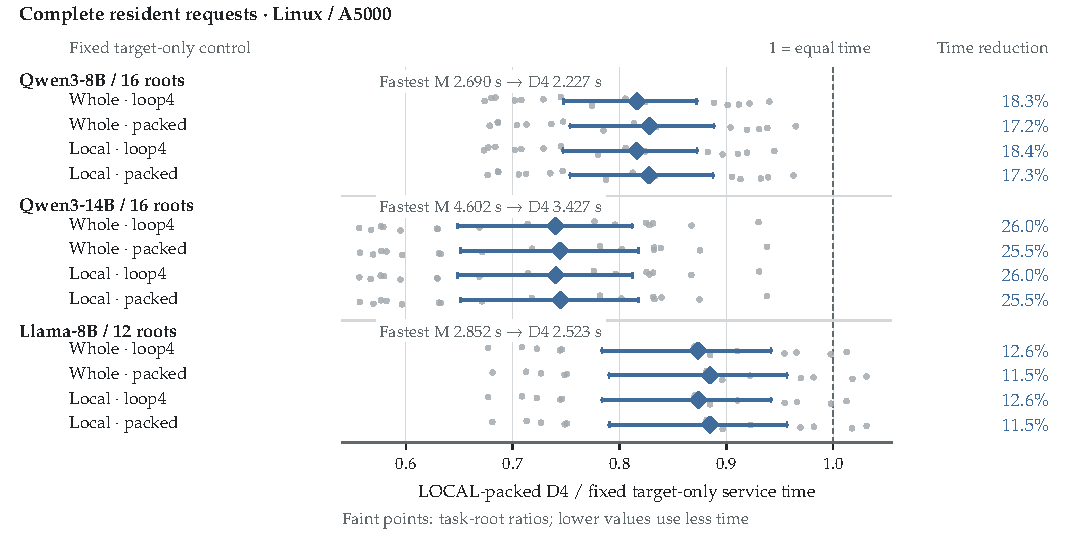
\includegraphics[width=\textwidth]{figures/service_controls.pdf}
\caption{Linux/A5000 resident service. Faint points show all task-root ratios. Each diamond compares LOCAL-packed D4 (draft prefill UB4, $k=3$) with a fixed target-only M; segments are 99\% paired-root intervals from the five-contrast family (the four M comparisons shown here and the W-L4-D4 comparison). Headers give fastest fixed M and D4 mean times. Qwen panels share 16 tasks; Llama has 12. Deployments are analyzed separately. Table~S1 reports all six arm means.}
\label{fig:service}
\end{figure*}

The 14B deployment also retains the benefit outside the internal service timer. The actual measured-request burst totals 294.632\,s for its strongest fixed M and 219.405\,s for LOCAL-packed D4, a 25.53\% reduction. Complete native-worker totals, including integrity checks, loading, primers and the request strings, change from 662.546 to 594.559\,s, a 10.26\% reduction. For Llama, resident requests benefit, while the recorded process-level total favors M for this short worker workload. Table~S2 reports resident and full-worker costs separately.

The Windows practical panel originally selected 16 task roots and retained all four target-only controls. LOCAL-packed D4 reduces resident service by 29.11\%, actual request-burst time by 29.09\% and worker-wall time by 26.00\%. Its complete phase account locates the savings primarily in continuation/verification. Supplement~S2 gives the absolute times and disjoint cost balance. The Linux Qwen panels reuse the Windows task records, while numerical references, measurements and deployment lifecycles are established separately.

Compatible target verification saves enough target work to cover draft work in these deployments. This gain belongs to the reference-compatible application, which whole-graph execution also supports. The balanced studies resolve the incremental effects of the two implementation choices.

\subsection{Balanced studies separate the sources of improvement}
\label{sec:factors}
The four-D4 factorial experiments hold the model, draft policy and transaction width fixed, then cross W/L cuts with loop4/packing. Every arm is remeasured in the same panel. Figure~\ref{fig:factorial} includes the root-level ratios and all four direct effects for both Qwen scales; the fifth member of the simultaneous-inference family is the root-level interaction reported in Supplement~S3.

\begin{figure*}[t]
\centering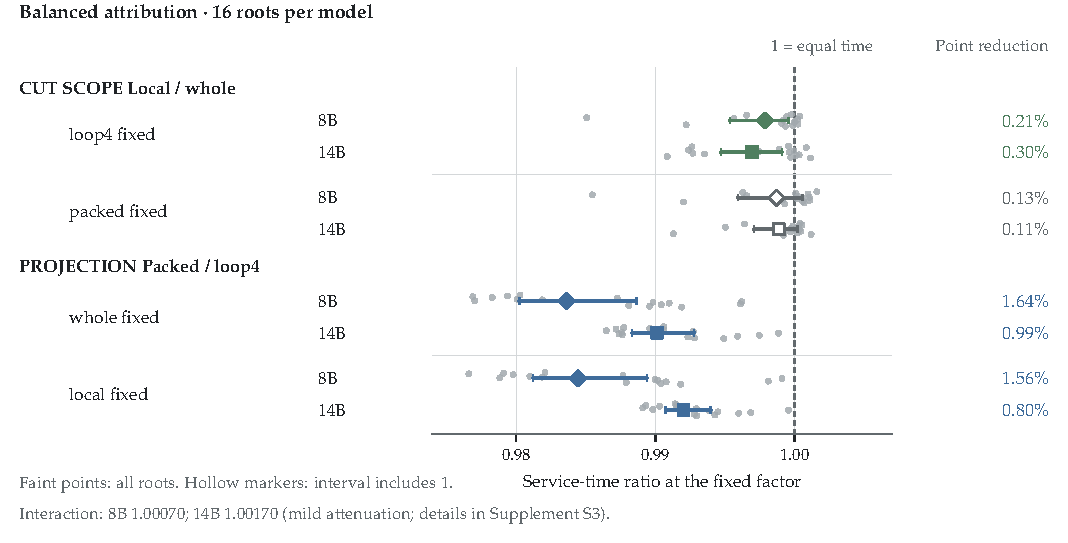
\includegraphics[width=\textwidth]{figures/factorial.pdf}
\caption{Balanced D4 attribution. Faint points show all 16 root ratios. Diamonds (8B) and squares (14B) mark complete-service total ratios; segments are 99\% adjusted intervals. Hollow, neutral markers identify intervals that include 1. The two sections isolate cut scope and projection. Table~S3 lists the fixed effects; Supplement~S3 defines the equal-root interaction.}
\label{fig:factorial}
\end{figure*}

At 8B, packing reduces service by 1.64\% with W and 1.56\% with L; at 14B, it saves 0.99\% and 0.80\%. Backend-loop4 already moves the simple loop out of the graph, so these comparisons measure the remaining packing increment.

At fixed loop4, local cuts save 0.21\% and 0.30\% for 8B and 14B. At fixed packing, the point reductions are 0.13\% and 0.11\%, with intervals containing 1. The interactions, 1.000696 and 1.001703, indicate mild attenuation when the two optimizations are combined.

The physical execution explains the scale of the cut effect. In the 8B factorial, 20 of 2,224 logical verification cycles require an extra whole-graph boundary split, approximately 0.899\%. LOCAL executes 2,224 four-row graphs and W executes 2,244 verification graphs, with the same number of target rows and the same prefill-width distribution. Local grouping avoids repeated graph work at those boundaries; most calls already have compatible geometry. The native observer places wide packing in prefill, not in four-row verification. This phase distinction explains where packing can contribute at $k=3$.

Packing organizes independent arithmetic groups, while local cuts preserve outer parallelism when a physical boundary divides a call. A deployment selects the implementations; per-call planning supplies their compatible groups.

\subsection{Typed grouping extends the method to 32B mixed quantization}
\label{sec:q4result}
The 32B deployment contains 385 Q4\_K, 65 Q6\_K and 257 F32 tensors. Its REF1 recipe is a typed extension: it retains scalar-column arithmetic for the mixed quantized projections and exposes independent columns as channels. All six paths pass finite vector/state checks before the four-root descriptive timing panel. The candidates share C1024, F16 KV, reserve 32 and a CUDA-Graphs-disabled policy. Transformer and output layers are GPU offloaded, with the standard CPU-mapped input embedding.

\begin{figure}[t]
\centering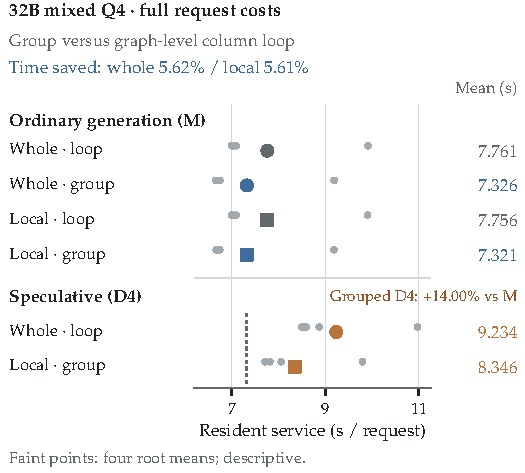
\includegraphics[width=\columnwidth]{figures/mixed_q4.pdf}
\caption{All six 32B mixed-Q4 paths. Markers and numbers give mean service; faint points are four exposed-root means over four rounds. Circles/squares distinguish whole/local scope. The loop control is graph-level scalar-column execution. Grouped D4 uses 14.00\% more time than the fastest M (dotted reference). Table~S4 reports complete costs.}
\label{fig:q4}
\end{figure}

Grouping reduces ordinary service from 124.183 to 117.208\,s with W fixed (5.62\%), and from 124.100 to 117.144\,s with L fixed (5.61\%), over 16 requests per arm. Both comparisons improve in all 16 matched root/round pairs. Worker totals fall by 3.98\% and 4.56\%, and caller totals by 3.85\% and 3.81\%, respectively. The grouped implementation retains scalar-column arithmetic while replacing separate column graphs and concatenation with one operation over independent channels.

Figure~\ref{fig:q4} identifies target-only grouped execution as the appropriate measured application choice. The grouped D4 path improves on the graph-loop D4 path, but takes 14.00\% more resident time than the fastest M. The ordinary-generation comparison fixes cut scope and excludes draft work, isolating the measured grouping package. A subsequent operand-level comparison with a backend-internal loop is reported in Supplement~S3.



\subsection{Physical geometry determines the value of local cuts}
The final Vulkan interface supports actual C1024 and C4096 allocations, the original prompt producer and known-query appends of 2, 4 and 32 rows. Figure~\ref{fig:vulkan} retains both within-bucket and crossing cases. In the six crossing coordinates, LOCAL reduces append time by 20.34\%--44.68\% relative to W. The paired inside controls are within approximately 0.43\%--3.74\% in the other direction.

\begin{figure}[t]
\centering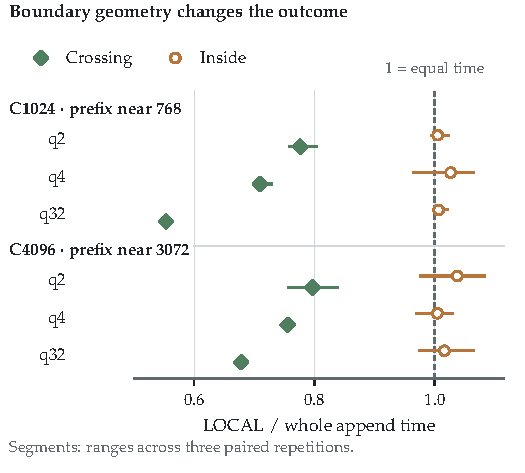
\includegraphics[width=\columnwidth]{figures/vulkan_geometry.pdf}
\caption{Vulkan append geometry. Filled diamonds denote crossings, hollow circles the inside controls, and the dashed line equal time. Segments show the minimum and maximum of the three observed paired ratios, not a population interval. Crossings split one row from the remainder. C1024 and C4096 jointly change capacity and active-prefix region.}
\label{fig:vulkan}
\end{figure}

Split geometry determines the work preserved by a local cut. Earlier q32 experiments used $16+16$ whole-graph splits and included cases favoring W; the final interface probes a $1+31$ split, one row before a physical boundary. The earlier full CUDA width/geometry matrix is reproduced in Supplement~S5. Its twelve fixed coordinates include cases where packing regresses, including Qwen crossing widths. The historical Vulkan cells are retained in Supplementary Fig.~S2. Natural alignment and whole-graph rechunking can make the schedules nearly coincide. Local grouping provides its benefit where it avoids fragmentation of the surrounding graph.

Vulkan executes two-query verification within the reference contract. In a separate resident mechanism window, LOCAL executes 578 occupied two-row target graphs for 1,156 rows, versus 1,156 scalar graphs in the earlier resident speculative path. Ordinary M executes 992 graphs for 992 rows. Batching reduces graph invocations while speculation changes the amount of target work. The complete pilot cost, including draft work, favors M in that deployment. The earlier natural-prefix AUTO panels on both RTX and B570 did not establish a service benefit over fixed policies; the strong whole-graph rechunk control can absorb much of the append-only gain. Supplement~S5 retains those separate negative controls and their lifecycles.

\subsection{Eight-row execution improves equal work; live width changes work}
\label{sec:width}
The $q=8$ implementation retains Q8\_0 weights and the arithmetic reference, extending the transaction to $k=7$ with candidate output reserve 8 for both widths. The width is physical: LOCAL can execute eight verification positions, while W splits according to actual extents. Original requested rows, pending/correction/bonus state, trim frontier and terminal handling are qualified against the independent reference.

\begin{figure*}[t]
\centering
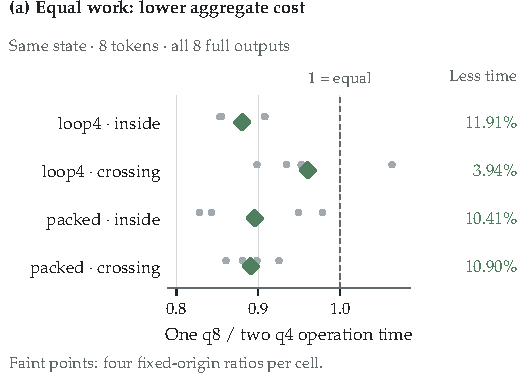
\includegraphics[width=.493\textwidth]{figures/width_equal.pdf}\hfill
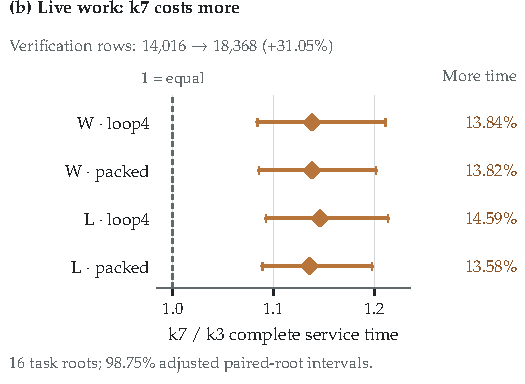
\includegraphics[width=.493\textwidth]{figures/width_live.pdf}
\caption{Equal-work efficiency and live workload. (a) One $q=8$ call versus two $q=4$ calls from the same state, using eight known tokens and all eight full outputs. Diamonds and percentages summarize total operation time; faint points retain all four origin ratios (one APPS, three GSM8K). (b) Four fixed-method $k=7$/$k=3$ service ratios from the separate 16-root live panel, with 98.75\% adjusted intervals; percentages denote increases. D4 is fixed; no contemporaneous M is timed.}
\label{fig:width}
\end{figure*}

Across the four development origins, one $q=8$ operation uses 3.94\%--11.91\% less aggregate time than two $q=4$ operations in the four RTX cells (Fig.~\ref{fig:width}a). Individual origin ratios remain visible, including the loop4-crossing origin above 1. The separate A5000 live pilot is reported in Supplement~S4.

In live generation, k7 reduces cycles from 3,504 to 2,296 per arm but increases verification rows from 14,016 to 18,368 for the same 11,472 emitted tokens. Acceptance among inspected proposals is 87.47\% and 87.93\%; acceptance among all proposals is 75.42\% and 56.94\%. The separate proposal accounts in the supplement distinguish actual mismatches from unconsumed suffixes.

All four complete-service width comparisons favor k3 by the ratios shown in Fig.~\ref{fig:width}b. For LOCAL-packed, $k=7$ adds 24.897\,s over 128 requests: verification adds 13.567\,s, draft proposal adds 13.224\,s, and draft synchronization saves 2.792\,s. Output copying contributes 0.252\,s; the remaining work closes the balance. Supplementary Fig.~S1 and Table~S6 preserve the decomposition and all eight arms.

The complete cost can be written as
\begin{equation}
 T_{\mathrm{spec}}=T_{\mathrm{target}}+T_{\mathrm{draft}}+T_{\mathrm{state/output/host}},
 \label{eq:cost}
\end{equation}
with disjoint intervals and a reconciled residual. Wider execution reduces some per-row cost, while longer proposals alter the total rows and consumed fraction. The evaluated live workload uses k3 as its effective fixed configuration; q8 remains a supported parallel execution capability with its own equal-work evidence.

\section{Related Work}
\label{sec:related}
\subsection{Preserving arithmetic across parallel execution}
Thinking Machines studies batch-invariant reduction choices for normalization, matrix multiplication and attention~\cite{thinkingmachines}. Taming reconstructs the bitwise arithmetic of existing cuBLAS kernels, enforces reduction descriptions during lowering and verifies compiled arithmetic properties~\cite{taming}. These works establish that existing numerical behavior can be an optimization target. Our contribution connects reference-compatible arithmetic to dense-cache prefixes, phase transitions and requested-output ownership in a quantized inference runtime. The native grouping recipes expose independent work while retaining the reference-sensitive organization within each group.

Public \texttt{llama\_reproducible} code includes a small-column quantized execution path~\cite{loop4code}. Backend-loop4 is therefore a direct performance control. The balanced experiments separate its remaining projection increment from cut scope. The mixed-Q4 study uses a scalar-column recipe and a different graph-level baseline, as summarized in Fig.~\ref{fig:q4}.

\subsection{System determinism and speculative execution}
Vosti studies engine-level determinism through formal relationships between engine state, cache behavior and kernel properties~\cite{vosti}. We study compatibility with an existing quantized deployment: phase-specific producers, physical cache geometry and qualified arithmetic determine the whole/local execution plans. Native numerical correspondence and complete-service measurements evaluate these plans.

LLM-42 uses a consistent verifier execution with verification and state repair~\cite{llm42}. Our supported paths organize compatible work before execution by binding offline-qualified arithmetic and cache requirements at each call. CoRun isolates prefill and uses fixed-shape batched decode for deterministic service~\cite{corun}. Phase plans instead expose row-dependent physical-prefix and output-state requirements, allowing attention-local cuts within a wider graph.

Speculative decoding and sampling reduce target invocations by evaluating proposals together~\cite{leviathan2023,chen2023}. Distribution preservation does not establish byte-identical finite-precision vectors and KV; the target-compatibility contract specifies those additional obligations. Draft width remains an application control. HeteroSpec allocates verification effort using contextual heterogeneity~\cite{liu2026heterospec}, a different objective from compatibility with a fixed deployment.
\section{Conclusion}
Reference-derived phase plans connect a deployment's numerical behavior to its parallel execution. They combine the producer history, physical KV range, type-specific arithmetic and ownership of logical outputs and state. Whole-graph and local-attention implementations place the cuts differently while preserving the reference-sensitive computation within each group.

CUDA and Vulkan studies support this approach across model structures, operating environments and quantized paths, including mixed-Q4 at 32B. Controlled comparisons separate packing's contribution from geometry-dependent local cuts. Complete requests then determine the useful deployment: speculative execution improves the three Linux service panels, grouped ordinary generation is preferable in the tested 32B configuration, and shorter proposals remain preferable in the live width study despite the aggregate equal-work advantage of eight-query execution. Phase plans make these choices available within an established numerical reference.

\section*{Acknowledgments}
OpenAI ChatGPT and Codex assisted with implementation, experiment and analysis tools, manuscript editing and figure code. The author is responsible for scientific interpretation and final approval.
\bibliographystyle{IEEEtran}
\bibliography{references}
\label{lastmainpage}
\ifdefined\includeSupplement
\clearpage
\setcounter{section}{0}
\setcounter{dbltopnumber}{3}
\renewcommand{\thesection}{S\arabic{section}}
\setcounter{table}{0}\renewcommand{\thetable}{S\arabic{table}}
\setcounter{figure}{0}\renewcommand{\thefigure}{S\arabic{figure}}
\begin{center}
{\Large Supplementary material}\\[4pt]
{\normalsize Reference-Compatible Parallel Execution for Quantized LLM Inference}
\end{center}

\section{Deployment and Evidence Register}
W/L denotes whole-graph/local-attention lowering; L4/P denotes the Q8 backend loop/packing implementation. M loads target resources only. D4 sets draft prefill UB4, independently of proposal count $k$. The 32B REF1-loop/group paths retain single-column Q4\_K/Q6\_K arithmetic. Tables retain every control and its cost window.

The profile is dense seq0, F16 K/V, greedy stopping and no FlashAttention. CUDA references use whole-prompt callers, physical UB1 and last-only output; Vulkan retains UB128 and its outer prompt calls. Each model/platform has its own R, including numerical modules, capacity, placement and output requests.

The Linux Qwen/Smol qualification records 6,740 requested full-vector comparisons and 4,784 active-state comparison records. Table~\ref{tab:panels} lists the task-root and repetition units separately.

Section~S6 and the companion manifest bind each result to its immutable source and reconstruction level.

\section{Complete Application and Lifecycle Costs}
\begin{table*}[t]
\centering\footnotesize\tighttable
\caption{All six Linux application arms: mean measured resident seconds per request. Qwen panels have 64 requests per arm; Llama has 48. Each has four sessions. The first four columns are genuine target-only controls.}
\label{tab:allservice}
\begin{tabular}{@{}lrrrrrr@{}}\toprule
Model & W-L4-M & W-P-M & L-L4-M & L-P-M & W-L4-D4 & L-P-D4\\\midrule
\ApplicationRows
\bottomrule\end{tabular}
\end{table*}

The Qwen panels share the same 16 task identities for deployment and scale transfer. The Llama study selects 12 roots using its recorded project-exposure exclusions. The three application analyses use ratios of totals and 10,000 paired-root bootstrap draws. Each five-comparison family includes L-P-D4 against every fixed M and W-L4-D4. The fastest fixed M provides a descriptive summary; the five registered contrasts supply the inference.

The first Linux 8B study uses four cyclic six-arm rows; W-L4-D4 precedes L-P-D4 in each. Its two-D4 difference changes both factors and retains potential order effects. The balanced four-D4 studies supply factor attribution independently. Llama and 14B use four rows of a six-arm design with partial position/neighbor coverage; their direct application comparisons retain that conditional scope.

\begin{table*}[t]
\centering\footnotesize\tighttable
\caption{Complete-cost windows for representative fixed controls. Each entry is an aggregate within one study. Resident service, measured-request burst, worker and caller clocks overlap and must not be added. A dash means that this table does not include that field, not a measured zero.}
\label{tab:costs}
\begin{tabularx}{\textwidth}{@{}L{2.35cm}L{2.30cm}rrrY@{}}\toprule
Deployment & Fixed comparison & Resident service (s) & Request burst (s) & Native workers (s) & Window interpretation\\\midrule
Linux Qwen3-8B & W-P-M / L-P-D4 & 172.146 / 142.523 & --- & 200.739 / 168.973 & Worker totals shown at reported millisecond precision.\\
Linux Qwen3-14B & W-P-M / L-P-D4 & 294.542 / 219.318 & 294.632 / 219.405 & 662.546 / 594.559 & Same registered requests; worker includes integrity, loading and primers.\\
Linux Llama-8B & L-P-M / L-P-D4 & 136.873 / 121.102 & --- & 361.717 / 368.822 & Resident improvement does not preserve the process-level ranking.\\
Windows Qwen3-8B & W-P-M / L-P-D4 & 219.810 / 155.814 & 220.178 / 156.126 & 260.240 / 192.568 & Windows measurements; task records reused for Linux, with separate references.\\\bottomrule
\end{tabularx}
\end{table*}

The Windows practical panel originally selected 16 new roots, four sessions, four real target-only M controls, one matched-residency M and L-P-D4. Its mean fixed-M times are 3.483689, 3.434533, 3.511301 and 3.474824\,s; L-P-D4 averages 2.434597\,s. The four-comparison adjusted root intervals support the reported resident-service direction. The added draft requires more initialization and sampled memory; its per-worker setup difference is approximately 0.420\,s and device-global sampled peak difference approximately 0.705\,GiB. The memory difference is a device-global sampled value; per-process peaks and energy were not measured.

The complete Windows 64-request phase account gives target savings 96.889\,s, draft additions 31.931\,s and other net additions 0.962\,s, yielding 63.996\,s of resident savings. In the two-root synchronized Vulkan cost diagnostic, target savings 0.466681\,s are offset by draft additions 1.923330\,s and other additions 0.210582\,s. The synchronized diagnostic and the four-root clean Vulkan pilot use distinct measurement windows and are reported separately.

\section{Factorial and Mixed-Q4 Results}
\begin{table}[t]
\centering\footnotesize\tighttable
\caption{All fixed effects from the balanced Qwen D4 panels. Ratios below 1 favor the numerator; intervals are 99\% family-adjusted paired-root percentiles. P denotes packing.}
\begin{tabular}{@{}llrl@{}}\toprule
Model & Fixed-factor comparison & Ratio & Interval\\\midrule
\FactorRows
\bottomrule\end{tabular}
\end{table}

Each factorial uses the same 16 task roots, four arms and four Williams rows, with two separate primers per worker: 256 formal requests plus 32 primers. The per-session arm orders balance all four positions and all 12 directed within-session neighbors. The interaction estimand is the equal-root geometric mean of $(L_P/W_P)/(L_{L4}/W_{L4})$. Its 8B estimate is 1.000696 with interval [1.000069, 1.001393]; the 14B estimate is 1.001703 with interval [1.000293, 1.003338]. Both interactions indicate mild attenuation of the combined effect. Figure~\ref{fig:factorial} includes every root-level ratio.

\begin{table*}[t]
\centering\footnotesize\tighttable
\caption{Complete 32B mixed-Q4 costs. Each arm has 16 measured requests and 16 full identical-root immediate warmups. Worker and caller totals include the warmups and initialization. They are not additional independent task observations.}
\label{tab:q32all}
\begin{tabular}{@{}lrrrr@{}}\toprule
Arm & Measured service sum (s) & Mean service (s) & Native-worker sum (s) & Caller sum (s)\\\midrule
\QThreeTwoRows
\bottomrule\end{tabular}
\end{table*}

The 32B reference is pristine Linux scalar execution with UB1/reserve 1. The candidates use UB32/reserve 32, C1024, F16 KV, no flash and a common graphs-disabled policy fixed before timing. The graph-level REF1-loop and independent REF1-group retain the per-type scalar dot functions and the original activation quantizer. The 5.61\% comparison uses graph-level scalar-column execution. The precise candidate source modification is in graph lowering; unchanged CUDA archive members are bound in the build record. Each requested full output and active state in the finite qualification is checked against this deployment's own reference.

The four exposed roots are short mathematics inputs. Whole/group and local/group improve ordinary service by 5.616\% and 5.606\% relative to their respective graph-level loops. At fixed projection, L/W differs by approximately 0.055\%--0.067\%. L-REF1-group-D4 takes 9.614\% less service than W-REF1-loop-D4, a compound comparison, but 14.000\% more than the strongest M. Table~\ref{tab:q32all} includes all six paths. Model size, quantization, recipe and graph policy jointly distinguish this deployment from the 14B Q8 study.


\subsection{Backend-internal loop: completed operator follow-up}
The follow-up at \texttt{f419a89d} fixes whole lowering and scalar-column arithmetic. G loops in the graph; B quantizes once and dispatches scalar dots inside the backend; C groups independent columns. After S1 qualification (243 workers, 783 operations), S2 completes three matched blocks in four exposed tensor cells: 36 fresh workers, each with one warmup and one measurement, all with CUDA Graphs off.

\begin{table}[t]
\centering\footnotesize\tighttable
\caption{Strong-loop operator comparison. B/G and C/B are geometric means of three paired elapsed-time ratios. The final column gives the observed C/B minimum--maximum, not a confidence interval. All four exposed cells are shown.}
\label{tab:strong-operator}
\begin{tabular}{@{}llrrl@{}}\toprule
Type & Width & B/G & C/B & C/B range\\\midrule
\StrongSTwoRows
\bottomrule\end{tabular}
\end{table}

B/G and C/B have equal-cell geometric ratios of 0.6390 and 0.8528 (Table~\ref{tab:strong-operator}); Q6\_K/$q=4$ has mixed paired directions. These one-warmup operator results complement the 5.61\% graph-loop service comparison. The full-model B comparison and matched-history A5000 width follow-up have no performance results in this fixed version. The package recomputes cell summaries from public block ratios, separately from the source authors' raw-time replay.

\section{Verification Width}
\begin{table}[t]
\centering\footnotesize\tighttable
\caption{All eight Windows width-study arms. Each arm has 128 formal requests: 16 roots across eight order blocks. The candidate output reservation is 8 for both k3 and k7.}
\begin{tabular}{@{}lrr@{}}\toprule
Arm & Service sum (s) & Mean (s)\\\midrule
\QEightRows
\bottomrule\end{tabular}
\end{table}

\begin{table}[t]
\centering\footnotesize\tighttable
\caption{Registered fixed-k7 secondary comparisons. Their 98.75\% adjusted intervals belong to a separate four-comparison family and all contain 1.}
\begin{tabular}{@{}lrl@{}}\toprule
Comparison & Ratio & Interval\\\midrule
\QEightSecondaryRows
\bottomrule\end{tabular}
\end{table}

\begin{figure}[t]
\centering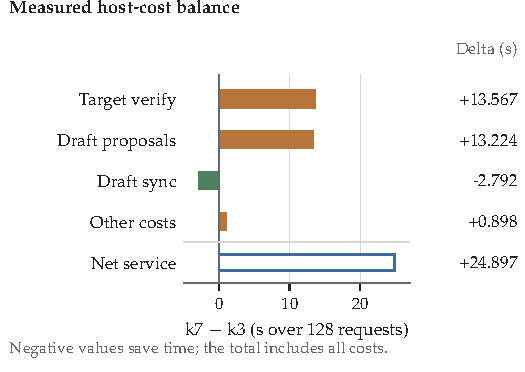
\includegraphics[width=\columnwidth]{figures/supp_width_cost.pdf}
\caption{LOCAL-packed host-cost difference over 128 requests. Bars and values give k7 minus k3; negative values save time. Other costs include prefill, output ownership, setup/teardown and the remaining residual. These measured phases include host work, synchronization and GPU execution.}
\label{fig:s-widthcost}
\end{figure}

Each arm emits 11,472 tokens. The corresponding k3/k7 counts are 3,504/2,296 verification cycles, 10,512/16,072 proposed tokens, 7,928/9,152 accepted proposals, 1,136/1,256 first inspected mismatches and 1,448/5,664 unconsumed suffix tokens. There are 14,016/18,368 verification rows and 28,416/32,768 total target rows. Native cap/EOG counts are 104/24 in each arm. Unconsumed suffixes include both post-rejection and terminal-boundary work, whose separate contributions are not resolved by these aggregate counts.

Dividing LOCAL-packed verification time by its row count gives a 9.68\% decrease per row, alongside 31.05\% more rows. The equal-work study instead holds state, eight known tokens and all eight full outputs constant. Its exposed origins are APPS/train/65 and GSM8K/test/70, /806 and /986. The protocol binds these origins and scalar continuations before timing; four AB/BA paired repetitions are diagnostics, separate from the 16-root live cohort. Its four aggregate ratios are 0.880898, 0.960562, 0.895916 and 0.890962 for loop4-inside, loop4-crossing, packed-inside and packed-crossing. Figure~\ref{fig:width}a displays all four cells and their origin-level ratios.

The original clean width panel retains all 1,024 measurements and 128 live primers. The complete performance source/input/order/statistics manifests preceded clean measurements; some earlier qualification fixtures were frozen in stages. A post-native mask-reader correction reused the unchanged first worker after offline validation, without a GPU rerun, and its inter-worker gap remains in the cost record. Later joint boundary/rollback qualification on an exposed natural root adds 1,936 full-vector and 296 active-target-KV comparisons across all eight arms. These comparisons cover the newly observed state transitions; the earlier clean runs retain their original endpoint and trace observations.

\subsection{A5000 live pilot and subsequent startup diagnostic}
The completed A5000 pilot at commit \texttt{2d076402} uses four exposed roots with cap 128, two live rounds and eight arms: 64 measurements and 32 primers. Table~\ref{tab:ampere-pilot} gives every live arm. LOCAL-packed $k=7$/$k=3$ service is 1.140572, while packed/loop4 at fixed LOCAL and $k=7$ is 0.981741. Verification time falls by 2.28\% in the latter comparison. The pilot is descriptive; it establishes the measured trade-off on those four inputs. A separate 32-measurement proposal-tape replay performs no draft work and has different target-row counts between widths.

\begin{table}[t]
\centering\footnotesize\tighttable
\caption{Completed A5000 live pilot, separate from the later first-use diagnostic. Each entry is the service total for eight requests (four roots, two rounds); D4 is fixed and both widths use reserve 8. Full precision and source identities accompany the manuscript.}
\label{tab:ampere-pilot}
\begin{tabular}{@{}lrr@{}}\toprule
Cut / projection & $k=3$ (s) & $k=7$ (s)\\\midrule
\AmperePilotRows
\bottomrule\end{tabular}
\end{table}

The subsequent A5000 equal-work follow-up uses unmatched first-use histories in one phase. Its measurements describe startup behavior and are kept separate from the completed live pilot and the RTX equal-work results. Matched-history A5000 timing has no completed result in this revision.

\section{Structural Geometry and Earlier Controls}


The final C1024/C4096 Vulkan append study records 12 coordinates, three paths and three repeats, giving 108 measured operations and 108 corresponding warmups. All allocated capacities and requested-output rules are checked natively. q32 retains the registered last-only output mask and copies the final requested vocabulary vector. The timer begins after valid state preparation and includes native phase binding, decode, synchronization and copied requested output. Caller batch preparation and state import are accounted separately.

In the Vulkan resident pilot, LOCAL uses 578 target graphs for 1,156 rows and W uses 582 graphs for those rows; M uses 992 scalar graphs/rows. On four exposed roots, the fastest speculative mean is 1.8235\,s versus 1.1503\,s for M, so this deployment favors ordinary generation.


\subsection{Archived structural and producer controls}
\label{supp:archive}
Table~\ref{tab:all-rtx-cells} gives the complete Qwen/Smol matrix across q4/q8/q32 and two physical ranges, with two known-token append repeats per cell. Packing improves some cells and regresses in others. q4 does not enter the wide packing route, so its timing differences are not attributed to that kernel.

\begin{table*}[t]
\centering\footnotesize\tighttable
\caption{Complete archived RTX known-query structural panel. Values are mean append milliseconds over two repetitions; W and L denote whole and local cut placement. L4 is backend-loop4 and P is independent-group packing. These fixed coordinates are separate from the sixteen-root natural D4 factorial.}
\label{tab:all-rtx-cells}
\begin{tabular}{@{}lrrrrrrrr@{}}\toprule
 & \multicolumn{4}{c}{Qwen3-8B} & \multicolumn{4}{c}{SmolLM2-1.7B}\\
\cmidrule(lr){2-5}\cmidrule(lr){6-9}
Geometry & W--L4 & W--P & L--L4 & L--P & W--L4 & W--P & L--L4 & L--P\\\midrule
q4 / inside & 25.35 & 27.77 & 27.23 & 27.33 & 7.64 & 7.70 & 7.74 & 7.77 \\
q4 / crossing & 41.76 & 49.28 & 25.28 & 29.78 & 14.18 & 14.34 & 9.16 & 9.69 \\
q8 / inside & 40.60 & 46.11 & 40.84 & 46.17 & 12.48 & 11.48 & 12.68 & 11.40 \\
q8 / crossing & 59.48 & 73.48 & 42.93 & 48.51 & 19.27 & 21.08 & 13.65 & 12.88 \\
q32 / inside & 149.19 & 158.82 & 168.04 & 159.56 & 45.65 & 33.00 & 41.40 & 33.02 \\
q32 / crossing & 167.24 & 188.30 & 161.62 & 163.33 & 46.67 & 43.03 & 42.22 & 34.96 \\
\bottomrule\end{tabular}
\end{table*}

\begin{table*}[t]
\centering\footnotesize\tighttable
\caption{Immutable experimental versions. Linked commits identify source trees; the accompanying manifest provides full paths, hashes and figure-input mappings.}
\label{tab:source-versions}
\begin{tabularx}{\textwidth}{@{}YlYl@{}}\toprule
Evidence & Commit & Evidence & Commit\\\midrule
CUDA prefix repair & \href{https://github.com/leecdiang/HeteroSpec/tree/e11d2b75d82422409ba2b701aa38c59f36acc50b}{\texttt{e11d2b75}} & Qwen3-14B service & \href{https://github.com/leecdiang/HeteroSpec/tree/0e9bb82432dc0a860a43ab9ba1c034f41176fe05}{\texttt{0e9bb824}} \\
Vulkan arithmetic/prefix repair & \href{https://github.com/leecdiang/HeteroSpec/tree/10a70566ce01ab707dbdcc57d8270c1434088f07}{\texttt{10a70566}} & Qwen3-14B balanced factors & \href{https://github.com/leecdiang/HeteroSpec/tree/44ef9b6654cfe3a800059d7311f8ecf73ffd8983}{\texttt{44ef9b66}} \\
Windows resident service & \href{https://github.com/leecdiang/HeteroSpec/tree/873d16712fbf3bc04f54e9b3753515c5dbebb60f}{\texttt{873d1671}} & A5000 four-root live pilot & \href{https://github.com/leecdiang/HeteroSpec/tree/2d076402b4ddc29c92549d360cd974af40d3f0a4}{\texttt{2d076402}} \\
Vulkan C1024/C4096 append & \href{https://github.com/leecdiang/HeteroSpec/tree/0575a34a88acff8298191e172205bf8726fe4174}{\texttt{0575a34a}} & RTX eight-query experiments & \href{https://github.com/leecdiang/HeteroSpec/tree/ba5b4c8e01d50d4bfaab1ac3908f798347be063a}{\texttt{ba5b4c8e}} \\
Linux Qwen3-8B service & \href{https://github.com/leecdiang/HeteroSpec/tree/592abdfe9267fd97ecbde18cd0ee9a1bfc319e20}{\texttt{592abdfe}} & q8 crossing-state extension & \href{https://github.com/leecdiang/HeteroSpec/tree/29a3751f3745668f287a8dcc3b2ad2c0d15bdc43}{\texttt{29a3751f}} \\
Qwen3-8B balanced factors & \href{https://github.com/leecdiang/HeteroSpec/tree/55f501e9a93013a4b4d82cc4967e82b8d9054a81}{\texttt{55f501e9}} & 32B mixed-Q4 deployment & \href{https://github.com/leecdiang/HeteroSpec/tree/41ef4ca6bbc382c02fb97ebea874651fbf9fd4ac}{\texttt{41ef4ca6}} \\
Llama final-method transfer & \href{https://github.com/leecdiang/HeteroSpec/tree/8990a80da23f75c071d6d161c8c79a2dc1347bd7}{\texttt{8990a80d}} & 32B strong-loop operators & \href{https://github.com/leecdiang/HeteroSpec/tree/f419a89d54f4ec93b4c9c328b4ea9f416ae3c989}{\texttt{f419a89d}} \\
\bottomrule
\end{tabularx}
\end{table*}

\begin{figure*}[t]
\centering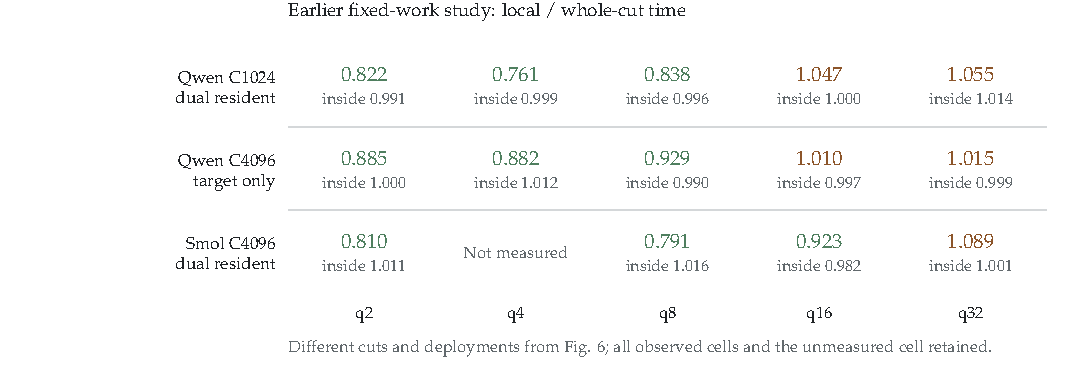
\includegraphics[width=\textwidth]{figures/supp_historical_geometry.pdf}
\caption{Archived Vulkan fixed-work layout geometry. Each labelled cell gives its measured crossing ratio and paired within-bucket control. A grey unmeasured cell is retained as missing, rather than interpolated. This historical configuration differs from the final resident C4096 experiment of Fig.~\ref{fig:vulkan}.}
\label{fig:historical-vulkan}
\end{figure*}

The RTX and B570 natural-prefix panels each use 32 held-out roots and four sessions. Both frozen AUTO policies are constant; neither meets its service-benefit screen, and all three baseline/AUTO intervals include 1. Their file-backed and host-memory snapshot lifecycles remain separate. A subsequent RTX study selects eight unexposed roots with distinguishing whole/rechunk calls before outputs. WB-rechunk/QB is 0.960486 for append and 0.994379 for complete service, with reversed service directions across sessions. These findings motivate the strong whole-rechunk control.

The B570 producer intervention uses eight preselected GSM8K~\cite{gsm8k}/MATH-500 roots, 48 scientific cells and 152 requests. P1-to-P4T changes initial full vectors and serialized state on all eight inputs; consumer compatibility depends on the resulting state, and some pairs still differ from the free reference. In the independent RTX witness, a 704-token prompt yields matching text but different active KV/frontier. A diagnostic $1+3$ split restores the scalar result; it supplies state evidence rather than a new service measurement.



\section{Sources and Reproduction}


The repository~\cite{records} supplies build/recipe histories, protocols, complete control records and statistical reconstructions. Model hashes bind licensed weight files. The manuscript package regenerates figures and tables from fixed projections, recomputes all 96 mixed-Q4 measurements and 16 registered $q=8$ interval endpoints from 128 arm/root aggregates, and identifies inherited intervals separately.

For the 8B factorial, 64 supplied W-L4 request times anchor other arm/root sums recovered from published paired ratios; these reproduce its four direct intervals and interaction. The 14B root ratios reproduce the interaction only. Added session and leave-one-root-out summaries are descriptive sensitivity checks. None changes the primary estimator or multiplicity family.

Weights and some large vector/KV captures remain in licensed or private storage. Independent numerical replication requires those inputs and new GPU execution; public-byte and statistical reconstruction alone does not perform it. Failed epochs, reader corrections and accounting remain in the repository. New recipes, devices or capacities bind a reference and requalify the affected operations.

\fi
\end{document}
